% Options for packages loaded elsewhere
\PassOptionsToPackage{unicode}{hyperref}
\PassOptionsToPackage{hyphens}{url}
%
\documentclass[
]{book}
\usepackage{amsmath,amssymb}
\usepackage{lmodern}
\usepackage{iftex}
\ifPDFTeX
  \usepackage[T1]{fontenc}
  \usepackage[utf8]{inputenc}
  \usepackage{textcomp} % provide euro and other symbols
\else % if luatex or xetex
  \usepackage{unicode-math}
  \defaultfontfeatures{Scale=MatchLowercase}
  \defaultfontfeatures[\rmfamily]{Ligatures=TeX,Scale=1}
\fi
% Use upquote if available, for straight quotes in verbatim environments
\IfFileExists{upquote.sty}{\usepackage{upquote}}{}
\IfFileExists{microtype.sty}{% use microtype if available
  \usepackage[]{microtype}
  \UseMicrotypeSet[protrusion]{basicmath} % disable protrusion for tt fonts
}{}
\makeatletter
\@ifundefined{KOMAClassName}{% if non-KOMA class
  \IfFileExists{parskip.sty}{%
    \usepackage{parskip}
  }{% else
    \setlength{\parindent}{0pt}
    \setlength{\parskip}{6pt plus 2pt minus 1pt}}
}{% if KOMA class
  \KOMAoptions{parskip=half}}
\makeatother
\usepackage{xcolor}
\usepackage[top=1in,left=0.3in,right=0.3in,bottom=1in]{geometry}
\usepackage{color}
\usepackage{fancyvrb}
\newcommand{\VerbBar}{|}
\newcommand{\VERB}{\Verb[commandchars=\\\{\}]}
\DefineVerbatimEnvironment{Highlighting}{Verbatim}{commandchars=\\\{\}}
% Add ',fontsize=\small' for more characters per line
\usepackage{framed}
\definecolor{shadecolor}{RGB}{248,248,248}
\newenvironment{Shaded}{\begin{snugshade}}{\end{snugshade}}
\newcommand{\AlertTok}[1]{\textcolor[rgb]{0.94,0.16,0.16}{#1}}
\newcommand{\AnnotationTok}[1]{\textcolor[rgb]{0.56,0.35,0.01}{\textbf{\textit{#1}}}}
\newcommand{\AttributeTok}[1]{\textcolor[rgb]{0.77,0.63,0.00}{#1}}
\newcommand{\BaseNTok}[1]{\textcolor[rgb]{0.00,0.00,0.81}{#1}}
\newcommand{\BuiltInTok}[1]{#1}
\newcommand{\CharTok}[1]{\textcolor[rgb]{0.31,0.60,0.02}{#1}}
\newcommand{\CommentTok}[1]{\textcolor[rgb]{0.56,0.35,0.01}{\textit{#1}}}
\newcommand{\CommentVarTok}[1]{\textcolor[rgb]{0.56,0.35,0.01}{\textbf{\textit{#1}}}}
\newcommand{\ConstantTok}[1]{\textcolor[rgb]{0.00,0.00,0.00}{#1}}
\newcommand{\ControlFlowTok}[1]{\textcolor[rgb]{0.13,0.29,0.53}{\textbf{#1}}}
\newcommand{\DataTypeTok}[1]{\textcolor[rgb]{0.13,0.29,0.53}{#1}}
\newcommand{\DecValTok}[1]{\textcolor[rgb]{0.00,0.00,0.81}{#1}}
\newcommand{\DocumentationTok}[1]{\textcolor[rgb]{0.56,0.35,0.01}{\textbf{\textit{#1}}}}
\newcommand{\ErrorTok}[1]{\textcolor[rgb]{0.64,0.00,0.00}{\textbf{#1}}}
\newcommand{\ExtensionTok}[1]{#1}
\newcommand{\FloatTok}[1]{\textcolor[rgb]{0.00,0.00,0.81}{#1}}
\newcommand{\FunctionTok}[1]{\textcolor[rgb]{0.00,0.00,0.00}{#1}}
\newcommand{\ImportTok}[1]{#1}
\newcommand{\InformationTok}[1]{\textcolor[rgb]{0.56,0.35,0.01}{\textbf{\textit{#1}}}}
\newcommand{\KeywordTok}[1]{\textcolor[rgb]{0.13,0.29,0.53}{\textbf{#1}}}
\newcommand{\NormalTok}[1]{#1}
\newcommand{\OperatorTok}[1]{\textcolor[rgb]{0.81,0.36,0.00}{\textbf{#1}}}
\newcommand{\OtherTok}[1]{\textcolor[rgb]{0.56,0.35,0.01}{#1}}
\newcommand{\PreprocessorTok}[1]{\textcolor[rgb]{0.56,0.35,0.01}{\textit{#1}}}
\newcommand{\RegionMarkerTok}[1]{#1}
\newcommand{\SpecialCharTok}[1]{\textcolor[rgb]{0.00,0.00,0.00}{#1}}
\newcommand{\SpecialStringTok}[1]{\textcolor[rgb]{0.31,0.60,0.02}{#1}}
\newcommand{\StringTok}[1]{\textcolor[rgb]{0.31,0.60,0.02}{#1}}
\newcommand{\VariableTok}[1]{\textcolor[rgb]{0.00,0.00,0.00}{#1}}
\newcommand{\VerbatimStringTok}[1]{\textcolor[rgb]{0.31,0.60,0.02}{#1}}
\newcommand{\WarningTok}[1]{\textcolor[rgb]{0.56,0.35,0.01}{\textbf{\textit{#1}}}}
\usepackage{longtable,booktabs,array}
\usepackage{calc} % for calculating minipage widths
% Correct order of tables after \paragraph or \subparagraph
\usepackage{etoolbox}
\makeatletter
\patchcmd\longtable{\par}{\if@noskipsec\mbox{}\fi\par}{}{}
\makeatother
% Allow footnotes in longtable head/foot
\IfFileExists{footnotehyper.sty}{\usepackage{footnotehyper}}{\usepackage{footnote}}
\makesavenoteenv{longtable}
\usepackage{graphicx}
\makeatletter
\def\maxwidth{\ifdim\Gin@nat@width>\linewidth\linewidth\else\Gin@nat@width\fi}
\def\maxheight{\ifdim\Gin@nat@height>\textheight\textheight\else\Gin@nat@height\fi}
\makeatother
% Scale images if necessary, so that they will not overflow the page
% margins by default, and it is still possible to overwrite the defaults
% using explicit options in \includegraphics[width, height, ...]{}
\setkeys{Gin}{width=\maxwidth,height=\maxheight,keepaspectratio}
% Set default figure placement to htbp
\makeatletter
\def\fps@figure{htbp}
\makeatother
\setlength{\emergencystretch}{3em} % prevent overfull lines
\providecommand{\tightlist}{%
  \setlength{\itemsep}{0pt}\setlength{\parskip}{0pt}}
\setcounter{secnumdepth}{5}
\usepackage{booktabs}
% \usepackage{amsthm}
% \makeatletter
% \def\thm@space@setup{%
%   \thm@preskip=8pt plus 2pt minus 4pt
%   \thm@postskip=\thm@preskip
% }
% \makeatother
\ifLuaTeX
  \usepackage{selnolig}  % disable illegal ligatures
\fi
\usepackage[]{natbib}
\bibliographystyle{apalike}
\IfFileExists{bookmark.sty}{\usepackage{bookmark}}{\usepackage{hyperref}}
\IfFileExists{xurl.sty}{\usepackage{xurl}}{} % add URL line breaks if available
\urlstyle{same} % disable monospaced font for URLs
\hypersetup{
  pdftitle={The Principle of R Package GSClassifier},
  pdfauthor={Weibin Huang},
  hidelinks,
  pdfcreator={LaTeX via pandoc}}

\title{The Principle of R Package GSClassifier}
\author{Weibin Huang}
\date{2022-09-13}

\begin{document}
\maketitle

{
\setcounter{tocdepth}{1}
\tableofcontents
}
\hypertarget{prerequisites}{%
\chapter{Prerequisites}\label{prerequisites}}

This is a \emph{sample} book written in \textbf{Markdown}. You can use anything that Pandoc's Markdown supports, e.g., a math equation \(a^2 + b^2 = c^2\).

The \textbf{bookdown} package can be installed from CRAN or Github:

\begin{Shaded}
\begin{Highlighting}[]
\FunctionTok{install.packages}\NormalTok{(}\StringTok{"bookdown"}\NormalTok{)}
\CommentTok{\# or the development version}
\CommentTok{\# devtools::install\_github("rstudio/bookdown")}
\end{Highlighting}
\end{Shaded}

Remember each Rmd file contains one and only one chapter, and a chapter is defined by the first-level heading \texttt{\#}.

To compile this example to PDF, you need XeLaTeX. You are recommended to install TinyTeX (which includes XeLaTeX): \url{https://yihui.org/tinytex/}.

\hypertarget{pre2}{%
\chapter{Prerequisites2}\label{pre2}}

You can label chapter and section titles using \texttt{\{\#label\}} after them, e.g., we can reference Chapter \ref{pre2}. If you do not manually label them, there will be automatic labels anyway, e.g., Chapter \ref{pre2}.

Figures and tables with captions will be placed in \texttt{figure} and \texttt{table} environments, respectively.

\begin{Shaded}
\begin{Highlighting}[]
\FunctionTok{par}\NormalTok{(}\AttributeTok{mar =} \FunctionTok{c}\NormalTok{(}\DecValTok{4}\NormalTok{, }\DecValTok{4}\NormalTok{, .}\DecValTok{1}\NormalTok{, .}\DecValTok{1}\NormalTok{))}
\FunctionTok{plot}\NormalTok{(pressure, }\AttributeTok{type =} \StringTok{\textquotesingle{}b\textquotesingle{}}\NormalTok{, }\AttributeTok{pch =} \DecValTok{19}\NormalTok{)}
\end{Highlighting}
\end{Shaded}

\begin{figure}

{\centering 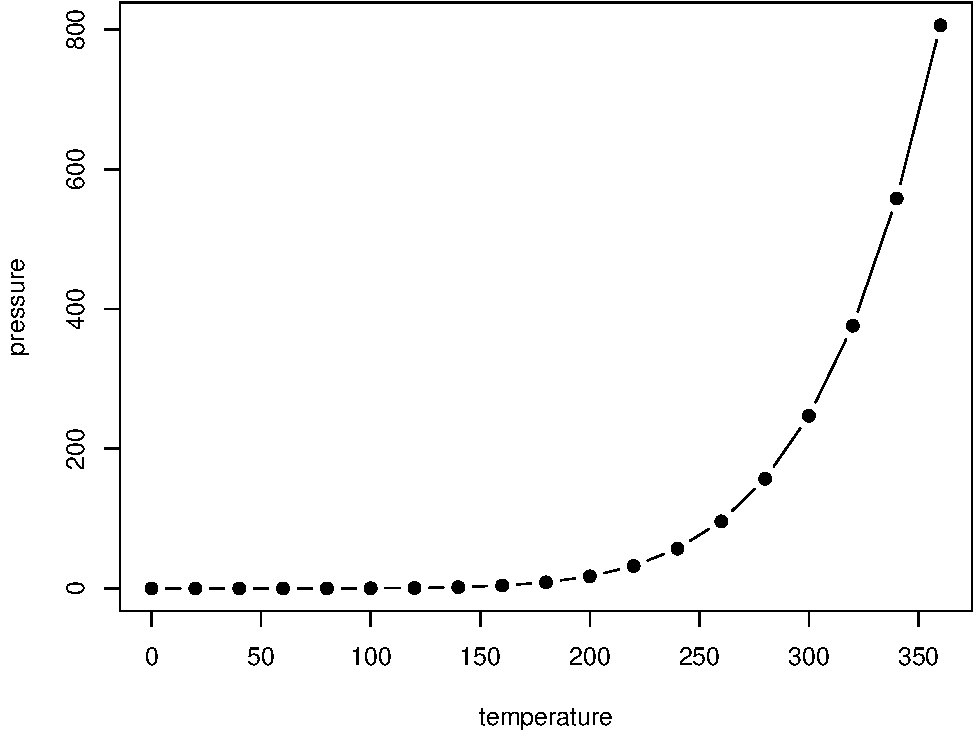
\includegraphics[width=0.8\linewidth]{index_files/figure-latex/nice-fig-1} 

}

\caption{Here is a nice figure!}\label{fig:nice-fig}
\end{figure}

Reference a figure by its code chunk label with the \texttt{fig:} prefix, e.g., see Figure \ref{fig:nice-fig}. Similarly, you can reference tables generated from \texttt{knitr::kable()}, e.g., see Table \ref{tab:nice-tab}.

\begin{Shaded}
\begin{Highlighting}[]
\NormalTok{knitr}\SpecialCharTok{::}\FunctionTok{kable}\NormalTok{(}
  \FunctionTok{head}\NormalTok{(iris, }\DecValTok{20}\NormalTok{), }\AttributeTok{caption =} \StringTok{\textquotesingle{}Here is a nice table!\textquotesingle{}}\NormalTok{,}
  \AttributeTok{booktabs =} \ConstantTok{TRUE}
\NormalTok{)}
\end{Highlighting}
\end{Shaded}

\begin{table}

\caption{\label{tab:nice-tab}Here is a nice table!}
\centering
\begin{tabular}[t]{rrrrl}
\toprule
Sepal.Length & Sepal.Width & Petal.Length & Petal.Width & Species\\
\midrule
5.1 & 3.5 & 1.4 & 0.2 & setosa\\
4.9 & 3.0 & 1.4 & 0.2 & setosa\\
4.7 & 3.2 & 1.3 & 0.2 & setosa\\
4.6 & 3.1 & 1.5 & 0.2 & setosa\\
5.0 & 3.6 & 1.4 & 0.2 & setosa\\
\addlinespace
5.4 & 3.9 & 1.7 & 0.4 & setosa\\
4.6 & 3.4 & 1.4 & 0.3 & setosa\\
5.0 & 3.4 & 1.5 & 0.2 & setosa\\
4.4 & 2.9 & 1.4 & 0.2 & setosa\\
4.9 & 3.1 & 1.5 & 0.1 & setosa\\
\addlinespace
5.4 & 3.7 & 1.5 & 0.2 & setosa\\
4.8 & 3.4 & 1.6 & 0.2 & setosa\\
4.8 & 3.0 & 1.4 & 0.1 & setosa\\
4.3 & 3.0 & 1.1 & 0.1 & setosa\\
5.8 & 4.0 & 1.2 & 0.2 & setosa\\
\addlinespace
5.7 & 4.4 & 1.5 & 0.4 & setosa\\
5.4 & 3.9 & 1.3 & 0.4 & setosa\\
5.1 & 3.5 & 1.4 & 0.3 & setosa\\
5.7 & 3.8 & 1.7 & 0.3 & setosa\\
5.1 & 3.8 & 1.5 & 0.3 & setosa\\
\bottomrule
\end{tabular}
\end{table}

You can write citations, too. For example, we are using the \textbf{bookdown} package in this sample book, which was built on top of R Markdown and \textbf{knitr} \citep{xie2015}.

\hypertarget{intro}{%
\chapter{Introduction}\label{intro}}

\href{https://github.com/huangwb8/GSClassifier}{GSClassifier} is an R package for modeling and identification of gene expression profiles (GEPs) subtypes. The detail of usage had been demonstrated in \href{https://github.com/huangwb8/GSClassifier/wiki}{Github WiKi}. Here, we propose to introduce the principle of GSClassifier, including flowchart, \textbf{top scoring pairs (TSP)} algorithm, and batch effect control.

\hypertarget{flowchart}{%
\chapter{Flowchart}\label{flowchart}}

Here is the flowchart of \texttt{GSClassifier}:

\begin{Shaded}
\begin{Highlighting}[]
\NormalTok{knitr}\SpecialCharTok{::}\FunctionTok{include\_graphics}\NormalTok{(}\FunctionTok{rep}\NormalTok{(}\StringTok{"./fig/flowchart.png"}\NormalTok{, }\DecValTok{1}\NormalTok{))}
\end{Highlighting}
\end{Shaded}

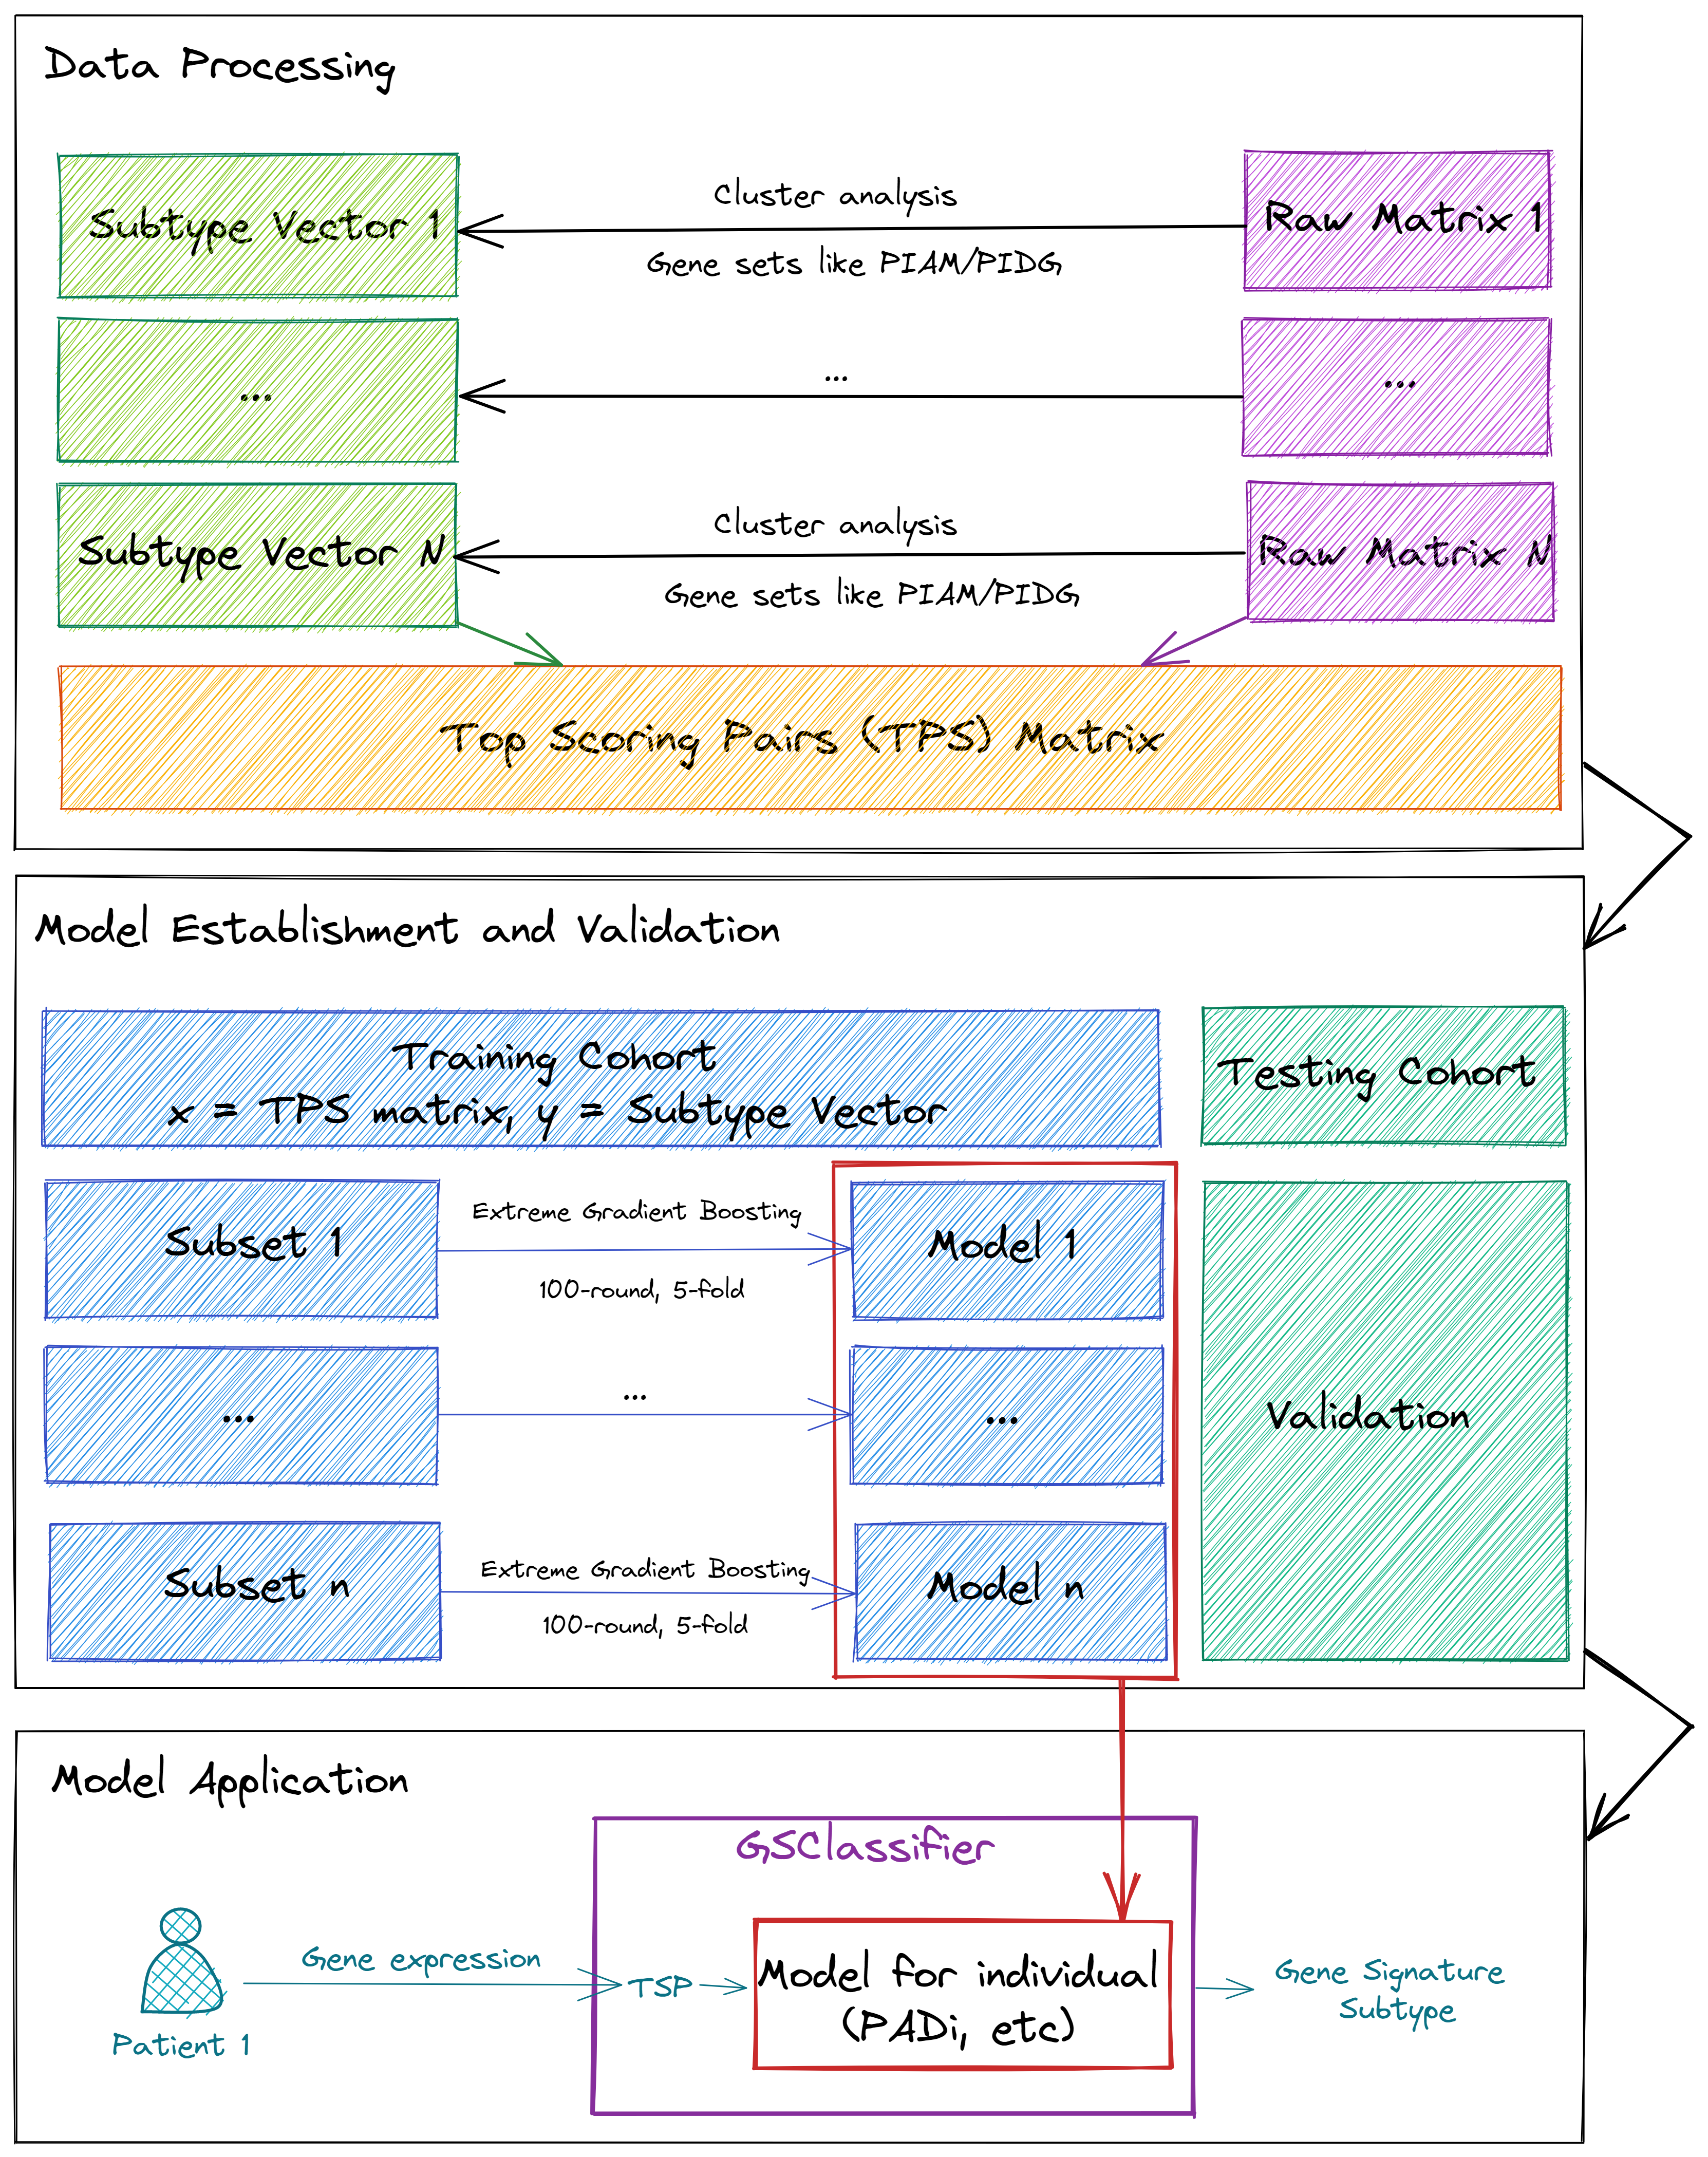
\includegraphics[width=46.18in]{./fig/flowchart}

\hypertarget{data-processing}{%
\section{Data Processing}\label{data-processing}}

For each dataset, the RNA expression matrix would be normalized (we called \texttt{Raw\ Matrix} in the flowchart) internally so that the expression data of the samples in the dataset were comparable.

Next, the subtypes of the samples in each dataset would be called based on cluster analysis. Specially, we figured out PAD subtypes, which belong to \texttt{Subtype\ Vector} in the flowchart, via hierarchical clustering analysis.

\hypertarget{top-scoring-pairs-tsp-matrix}{%
\section{Top scoring pairs (TSP) matrix}\label{top-scoring-pairs-tsp-matrix}}

With \texttt{subtype\ vectors} and \texttt{Raw\ Matrix}, the TSP matrix for a specified subtypes could be calculated via function \texttt{GSClassifier::trainDataProc}:

\begin{Shaded}
\begin{Highlighting}[]
\FunctionTok{trainDataProc}\NormalTok{(}
\NormalTok{  Xmat, Yvec,}
  
\NormalTok{  geneSet, }

  \AttributeTok{subtype =} \DecValTok{1}\NormalTok{, }
  
  \CommentTok{\# 0.2 was Used in PAD project}
  \AttributeTok{ptail =} \FloatTok{0.2}\NormalTok{,}
  
  \CommentTok{\# c(0, 0.25, 0.5, 0.75, 1.0) was Used in PAD project}
  \AttributeTok{breakVec =} \FunctionTok{c}\NormalTok{(}\DecValTok{0}\NormalTok{, }\FloatTok{0.25}\NormalTok{, }\FloatTok{0.5}\NormalTok{, }\FloatTok{0.75}\NormalTok{, }\FloatTok{1.0}\NormalTok{)}
\NormalTok{)}
\end{Highlighting}
\end{Shaded}

The TSP matrix consists of 3 parts: \textbf{binned expression matrix}, \textbf{top scoring of gene pairs}, and \textbf{gene set pairs}.

Here, we would use some simulated data to introduce how TSP matrix calculated.

\hypertarget{dataset}{%
\subsection{Dataset}\label{dataset}}

Load packages:

\begin{Shaded}
\begin{Highlighting}[]
\CommentTok{\# Install "devtools" package}
\ControlFlowTok{if}\NormalTok{ (}\SpecialCharTok{!}\FunctionTok{requireNamespace}\NormalTok{(}\StringTok{"devtools"}\NormalTok{, }\AttributeTok{quietly =} \ConstantTok{TRUE}\NormalTok{))}
    \FunctionTok{install.packages}\NormalTok{(}\StringTok{"devtools"}\NormalTok{)}

\CommentTok{\# Install dependencies}
\ControlFlowTok{if}\NormalTok{ (}\SpecialCharTok{!}\FunctionTok{requireNamespace}\NormalTok{(}\StringTok{"luckyBase"}\NormalTok{, }\AttributeTok{quietly =} \ConstantTok{TRUE}\NormalTok{))}
\NormalTok{    devtools}\SpecialCharTok{::}\FunctionTok{install\_github}\NormalTok{(}\StringTok{"huangwb8/luckyBase"}\NormalTok{)}

\CommentTok{\# Install the "GSClassifier" package}
\ControlFlowTok{if}\NormalTok{ (}\SpecialCharTok{!}\FunctionTok{requireNamespace}\NormalTok{(}\StringTok{"GSClassifier"}\NormalTok{, }\AttributeTok{quietly =} \ConstantTok{TRUE}\NormalTok{))}
\NormalTok{    devtools}\SpecialCharTok{::}\FunctionTok{install\_github}\NormalTok{(}\StringTok{"huangwb8/GSClassifier"}\NormalTok{)}

\CommentTok{\# Install CRAN packages}
\ControlFlowTok{if}\NormalTok{ (}\SpecialCharTok{!}\FunctionTok{requireNamespace}\NormalTok{(}\StringTok{"pacman"}\NormalTok{, }\AttributeTok{quietly =} \ConstantTok{TRUE}\NormalTok{))\{}
  \FunctionTok{install.packages}\NormalTok{(}\StringTok{"pacman"}\NormalTok{)}
  \FunctionTok{library}\NormalTok{(pacman)}
\NormalTok{\} }\ControlFlowTok{else}\NormalTok{ \{}
  \FunctionTok{library}\NormalTok{(pacman)}
\NormalTok{\}}
\NormalTok{packages\_needed }\OtherTok{\textless{}{-}} \FunctionTok{c}\NormalTok{(}\StringTok{"readxl"}\NormalTok{,}\StringTok{"ComplexHeatmap"}\NormalTok{,}\StringTok{"GSClassifier"}\NormalTok{)}
\ControlFlowTok{for}\NormalTok{(i }\ControlFlowTok{in}\NormalTok{ packages\_needed)\{}\FunctionTok{p\_load}\NormalTok{(}\AttributeTok{char=}\NormalTok{i)\}}
\end{Highlighting}
\end{Shaded}

We simulated a dataset:

\begin{Shaded}
\begin{Highlighting}[]
\CommentTok{\# Geneset}
\NormalTok{geneSet }\OtherTok{\textless{}{-}} \FunctionTok{list}\NormalTok{(}
  \AttributeTok{Set1 =} \FunctionTok{paste}\NormalTok{(}\StringTok{\textquotesingle{}Gene\textquotesingle{}}\NormalTok{,}\DecValTok{1}\SpecialCharTok{:}\DecValTok{3}\NormalTok{,}\AttributeTok{sep =} \StringTok{\textquotesingle{}\textquotesingle{}}\NormalTok{),}
  \AttributeTok{Set2 =} \FunctionTok{paste}\NormalTok{(}\StringTok{\textquotesingle{}Gene\textquotesingle{}}\NormalTok{,}\DecValTok{4}\SpecialCharTok{:}\DecValTok{6}\NormalTok{,}\AttributeTok{sep =} \StringTok{\textquotesingle{}\textquotesingle{}}\NormalTok{)}
\NormalTok{)}


\CommentTok{\# RNA expression}
\NormalTok{x }\OtherTok{\textless{}{-}} \FunctionTok{read\_xlsx}\NormalTok{(}\StringTok{\textquotesingle{}./data/simulated{-}data.xlsx\textquotesingle{}}\NormalTok{, }\AttributeTok{sheet =} \StringTok{\textquotesingle{}RNA\textquotesingle{}}\NormalTok{); expr }\OtherTok{\textless{}{-}} \FunctionTok{as.matrix}\NormalTok{(x[,}\SpecialCharTok{{-}}\DecValTok{1}\NormalTok{]); }\FunctionTok{rownames}\NormalTok{(expr) }\OtherTok{\textless{}{-}} \FunctionTok{as.character}\NormalTok{(}\FunctionTok{as.matrix}\NormalTok{(x[,}\DecValTok{1}\NormalTok{])); }\FunctionTok{rm}\NormalTok{(x)}
\end{Highlighting}
\end{Shaded}

\begin{verbatim}
## New names:
\end{verbatim}

\begin{Shaded}
\begin{Highlighting}[]
\CommentTok{\# Parameters}
\NormalTok{breakVec }\OtherTok{=} \FunctionTok{c}\NormalTok{(}\DecValTok{0}\NormalTok{, }\FloatTok{0.25}\NormalTok{, }\FloatTok{0.5}\NormalTok{, }\FloatTok{0.75}\NormalTok{, }\FloatTok{1.0}\NormalTok{)}
\NormalTok{subtype\_vector }\OtherTok{=} \FunctionTok{c}\NormalTok{(}\DecValTok{1}\NormalTok{,}\DecValTok{1}\NormalTok{,}\DecValTok{1}\NormalTok{,}\DecValTok{2}\NormalTok{,}\DecValTok{2}\NormalTok{,}\DecValTok{2}\NormalTok{)}
\NormalTok{Ybin }\OtherTok{=} \FunctionTok{ifelse}\NormalTok{(subtype\_vector }\SpecialCharTok{==} \DecValTok{1}\NormalTok{, }\AttributeTok{yes =} \DecValTok{1}\NormalTok{, }\AttributeTok{no=}\DecValTok{0}\NormalTok{)}

\CommentTok{\# Report}
\FunctionTok{cat}\NormalTok{(}\FunctionTok{c}\NormalTok{(}\StringTok{\textquotesingle{}}\SpecialCharTok{\textbackslash{}n}\StringTok{\textquotesingle{}}\NormalTok{, }\StringTok{\textquotesingle{}Gene sets:\textquotesingle{}}\NormalTok{, }\StringTok{\textquotesingle{}}\SpecialCharTok{\textbackslash{}n}\StringTok{\textquotesingle{}}\NormalTok{))}
\end{Highlighting}
\end{Shaded}

\begin{verbatim}
## 
##  Gene sets:
\end{verbatim}

\begin{Shaded}
\begin{Highlighting}[]
\FunctionTok{print}\NormalTok{(geneSet)}
\end{Highlighting}
\end{Shaded}

\begin{verbatim}
## $Set1
## [1] "Gene1" "Gene2" "Gene3"
## 
## $Set2
## [1] "Gene4" "Gene5" "Gene6"
\end{verbatim}

\begin{Shaded}
\begin{Highlighting}[]
\FunctionTok{cat}\NormalTok{(}\StringTok{\textquotesingle{}RNA expression:\textquotesingle{}}\NormalTok{, }\StringTok{\textquotesingle{}}\SpecialCharTok{\textbackslash{}n}\StringTok{\textquotesingle{}}\NormalTok{)}
\end{Highlighting}
\end{Shaded}

\begin{verbatim}
## RNA expression:
\end{verbatim}

\begin{Shaded}
\begin{Highlighting}[]
\FunctionTok{print}\NormalTok{(expr)}
\end{Highlighting}
\end{Shaded}

\begin{verbatim}
##       Sample1 Sample2 Sample3 Sample4 Sample5 Sample6
## Gene1    0.51    0.52    0.60    0.21    0.30    0.40
## Gene2    0.52    0.54    0.58    0.22    0.31    0.35
## Gene3    0.53    0.60    0.61    0.23    0.29    0.30
## Gene4    0.21    0.30    0.40    0.51    0.52    0.60
## Gene5    0.22    0.31    0.35    0.52    0.54    0.58
## Gene6    0.23    0.29    0.30    0.53    0.60    0.61
## Gene7    0.10    0.12    0.09    0.11    0.12    0.14
\end{verbatim}

Have a look at the matrix:

\begin{Shaded}
\begin{Highlighting}[]
\FunctionTok{Heatmap}\NormalTok{(}\FunctionTok{t}\NormalTok{(}\FunctionTok{scale}\NormalTok{(}\FunctionTok{t}\NormalTok{(expr))), }\AttributeTok{name =} \StringTok{"Z{-}score"}\NormalTok{)}
\end{Highlighting}
\end{Shaded}

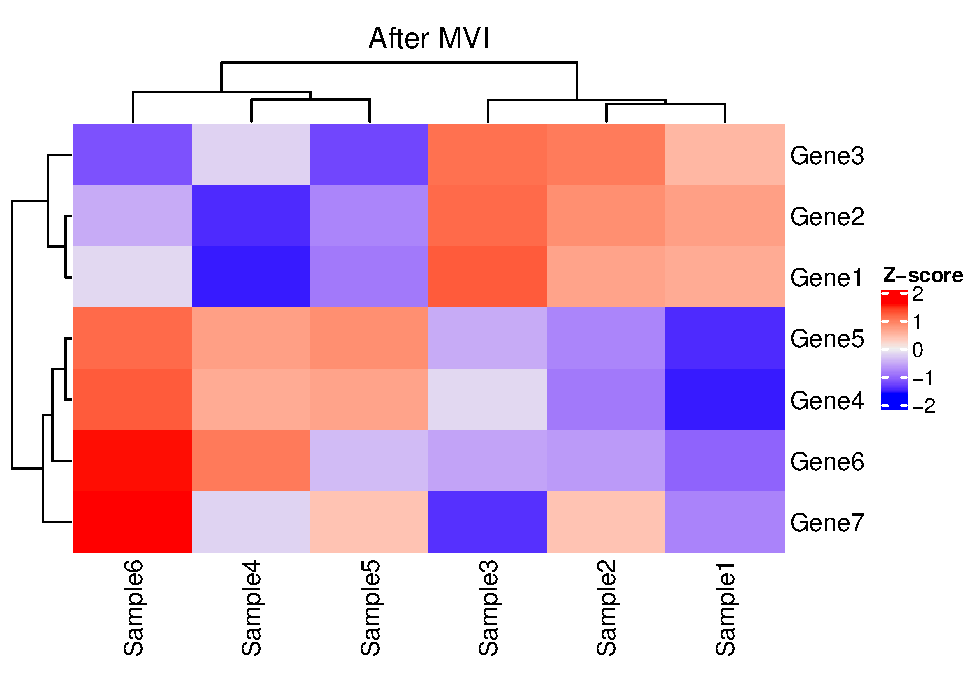
\includegraphics{Flowchart_files/figure-latex/unnamed-chunk-5-1.pdf}

\hypertarget{binned-expression}{%
\subsection{Binned expression}\label{binned-expression}}

\begin{Shaded}
\begin{Highlighting}[]
\CommentTok{\# Data of one sample}

\NormalTok{x }\OtherTok{\textless{}{-}}\NormalTok{ expr[,}\DecValTok{1}\NormalTok{]}

\CommentTok{\# Create quantiles  }
\NormalTok{brks }\OtherTok{\textless{}{-}} \FunctionTok{quantile}\NormalTok{(}\FunctionTok{as.numeric}\NormalTok{(x), }\AttributeTok{probs=}\NormalTok{breakVec, }\AttributeTok{na.rm =}\NormalTok{ T)}

\CommentTok{\# Get interval orders}
\NormalTok{xbin }\OtherTok{\textless{}{-}} \FunctionTok{.bincode}\NormalTok{(}\AttributeTok{x =}\NormalTok{ x, }\AttributeTok{breaks =}\NormalTok{ brks, }\AttributeTok{include.lowest =}\NormalTok{ T)}
\NormalTok{xbin }\OtherTok{\textless{}{-}} \FunctionTok{as.numeric}\NormalTok{(xbin)}

\CommentTok{\# Report}
\FunctionTok{cat}\NormalTok{(}\StringTok{\textquotesingle{}Quantiles:\textquotesingle{}}\NormalTok{, }\StringTok{\textquotesingle{}}\SpecialCharTok{\textbackslash{}n}\StringTok{\textquotesingle{}}\NormalTok{); }\FunctionTok{print}\NormalTok{(brks)}
\end{Highlighting}
\end{Shaded}

\begin{verbatim}
## Quantiles:
\end{verbatim}

\begin{verbatim}
##    0%   25%   50%   75%  100% 
## 0.100 0.215 0.230 0.515 0.530
\end{verbatim}

\begin{Shaded}
\begin{Highlighting}[]
\FunctionTok{cat}\NormalTok{(}\StringTok{\textquotesingle{}}\SpecialCharTok{\textbackslash{}n}\StringTok{\textquotesingle{}}\NormalTok{)}
\end{Highlighting}
\end{Shaded}

\begin{Shaded}
\begin{Highlighting}[]
\FunctionTok{cat}\NormalTok{(}\StringTok{\textquotesingle{}Raw expression:\textquotesingle{}}\NormalTok{, }\StringTok{\textquotesingle{}}\SpecialCharTok{\textbackslash{}n}\StringTok{\textquotesingle{}}\NormalTok{);}\FunctionTok{print}\NormalTok{(}\FunctionTok{as.numeric}\NormalTok{(x))}
\end{Highlighting}
\end{Shaded}

\begin{verbatim}
## Raw expression:
\end{verbatim}

\begin{verbatim}
## [1] 0.51 0.52 0.53 0.21 0.22 0.23 0.10
\end{verbatim}

\begin{Shaded}
\begin{Highlighting}[]
\FunctionTok{cat}\NormalTok{(}\StringTok{\textquotesingle{}}\SpecialCharTok{\textbackslash{}n}\StringTok{\textquotesingle{}}\NormalTok{)}
\end{Highlighting}
\end{Shaded}

\begin{Shaded}
\begin{Highlighting}[]
\FunctionTok{cat}\NormalTok{(}\StringTok{\textquotesingle{}Binned expression:\textquotesingle{}}\NormalTok{, }\StringTok{\textquotesingle{}}\SpecialCharTok{\textbackslash{}n}\StringTok{\textquotesingle{}}\NormalTok{); }\FunctionTok{print}\NormalTok{(xbin)}
\end{Highlighting}
\end{Shaded}

\begin{verbatim}
## Binned expression:
\end{verbatim}

\begin{verbatim}
## [1] 3 4 4 1 2 2 1
\end{verbatim}

For example, \texttt{0.10} is the minimun of the raw expression vector, so its binned expression is \texttt{1}. Similarly, the binned expression of maximum \texttt{0.53} is \texttt{4}.

We calculated binned expression via function \texttt{breakBin} in \texttt{GSClassifier}:

\begin{Shaded}
\begin{Highlighting}[]
\NormalTok{expr\_binned }\OtherTok{\textless{}{-}} \FunctionTok{apply}\NormalTok{(expr, }\DecValTok{2}\NormalTok{, }
\NormalTok{                 GSClassifier}\SpecialCharTok{:::}\NormalTok{breakBin,}
\NormalTok{                 breakVec)}
\FunctionTok{rownames}\NormalTok{(expr\_binned) }\OtherTok{\textless{}{-}} \FunctionTok{rownames}\NormalTok{(expr)}
\FunctionTok{print}\NormalTok{(expr\_binned)}
\end{Highlighting}
\end{Shaded}

\begin{verbatim}
##       Sample1 Sample2 Sample3 Sample4 Sample5 Sample6
## Gene1       3       3       4       1       2       2
## Gene2       4       4       3       2       2       2
## Gene3       4       4       4       2       1       1
## Gene4       1       2       2       3       3       4
## Gene5       2       2       2       4       4       3
## Gene6       2       1       1       4       4       4
## Gene7       1       1       1       1       1       1
\end{verbatim}

\hypertarget{genes-with-large-rank-differences}{%
\subsection{Genes with large rank differences}\label{genes-with-large-rank-differences}}

In this simulated dataset, \texttt{Gene7} is a gene whose expression is always the lowest across all samples. In other words, the rank of \texttt{Gene7} is stable or invariable across samples so that it's not robust for identification of differentail subtypes.

Except binned expression, we also calculated gene-pair scores later. Due to the number of gene-pair is \(C_{2 \atop n}\), the removement of genes like \texttt{Gene7} before modeling could really reduce the complexibility of the model and save computing resources. In all, genes like \texttt{Gene7} could be dropped out in the following analysis.

First, We use \texttt{base::rank}to return the sample ranks of the values in a vector:

\begin{Shaded}
\begin{Highlighting}[]
\NormalTok{expr\_binned\_rank }\OtherTok{\textless{}{-}} \FunctionTok{apply}\NormalTok{(}
\NormalTok{  expr\_binned, }
  \DecValTok{2}\NormalTok{, }
  \ControlFlowTok{function}\NormalTok{(x)}\FunctionTok{rank}\NormalTok{(x, }\AttributeTok{na.last =} \ConstantTok{TRUE}\NormalTok{)}
\NormalTok{)}
\FunctionTok{print}\NormalTok{(expr\_binned\_rank)}
\end{Highlighting}
\end{Shaded}

\begin{verbatim}
##       Sample1 Sample2 Sample3 Sample4 Sample5 Sample6
## Gene1     5.0     5.0     6.5     1.5     3.5     3.5
## Gene2     6.5     6.5     5.0     3.5     3.5     3.5
## Gene3     6.5     6.5     6.5     3.5     1.5     1.5
## Gene4     1.5     3.5     3.5     5.0     5.0     6.5
## Gene5     3.5     3.5     3.5     6.5     6.5     5.0
## Gene6     3.5     1.5     1.5     6.5     6.5     6.5
## Gene7     1.5     1.5     1.5     1.5     1.5     1.5
\end{verbatim}

\texttt{na.last\ =\ TRUE} means that missing values in the data are put last.

Then, get rank differences of each gene based on specified subtype distribution (\texttt{Ybin}):

\begin{Shaded}
\begin{Highlighting}[]
\NormalTok{testRes }\OtherTok{\textless{}{-}} \FunctionTok{sapply}\NormalTok{(}\DecValTok{1}\SpecialCharTok{:}\FunctionTok{nrow}\NormalTok{(expr\_binned\_rank), }\ControlFlowTok{function}\NormalTok{(gi) }\FunctionTok{testFun}\NormalTok{(}\FunctionTok{as.numeric}\NormalTok{(expr\_binned\_rank[gi,]), Ybin)); }\FunctionTok{names}\NormalTok{(testRes) }\OtherTok{\textless{}{-}} \FunctionTok{rownames}\NormalTok{(expr\_binned\_rank)}
\FunctionTok{print}\NormalTok{(testRes)}
\end{Highlighting}
\end{Shaded}

\begin{verbatim}
##     Gene1     Gene2     Gene3     Gene4     Gene5     Gene6     Gene7 
## -2.666667 -2.500000 -4.333333  2.666667  2.500000  4.333333  0.000000
\end{verbatim}

\texttt{Gene7} is the one with the lowest absolute value (0) of rank diffrence.

In \texttt{GSClassifier}, we use \texttt{ptail} to select differential genes based on rank diffrences. \textbf{Less \texttt{ptail} is, less gene kept}. Here, we just set \texttt{ptail=0.4}:

\begin{Shaded}
\begin{Highlighting}[]
\CommentTok{\# ptail is a numeber ranging (0,0.5].}
\NormalTok{ptail }\OtherTok{=} \FloatTok{0.4}

\CommentTok{\# Index of target genes with big rank differences}
\NormalTok{idx }\OtherTok{\textless{}{-}} \FunctionTok{which}\NormalTok{((testRes }\SpecialCharTok{\textless{}} \FunctionTok{quantile}\NormalTok{(testRes, ptail, }\AttributeTok{na.rm =}\NormalTok{ T)) }\SpecialCharTok{|}\NormalTok{ (testRes }\SpecialCharTok{\textgreater{}} \FunctionTok{quantile}\NormalTok{(testRes, }\FloatTok{1.0}\SpecialCharTok{{-}}\NormalTok{ptail, }\AttributeTok{na.rm =}\NormalTok{ T)))}

\CommentTok{\# Target genes}
\NormalTok{gene\_bigRank }\OtherTok{\textless{}{-}} \FunctionTok{names}\NormalTok{(testRes)[idx]}

\CommentTok{\# Report}
\FunctionTok{cat}\NormalTok{(}\StringTok{\textquotesingle{}Index of target genes: \textquotesingle{}}\NormalTok{,}\StringTok{\textquotesingle{}}\SpecialCharTok{\textbackslash{}n}\StringTok{\textquotesingle{}}\NormalTok{);}\FunctionTok{print}\NormalTok{(idx); }\FunctionTok{cat}\NormalTok{(}\StringTok{\textquotesingle{}}\SpecialCharTok{\textbackslash{}n}\StringTok{\textquotesingle{}}\NormalTok{)}
\end{Highlighting}
\end{Shaded}

\begin{verbatim}
## Index of target genes:
\end{verbatim}

\begin{verbatim}
## Gene1 Gene2 Gene3 Gene4 Gene5 Gene6 
##     1     2     3     4     5     6
\end{verbatim}

\begin{Shaded}
\begin{Highlighting}[]
\FunctionTok{cat}\NormalTok{(}\StringTok{\textquotesingle{}Target genes:\textquotesingle{}}\NormalTok{,}\StringTok{\textquotesingle{}}\SpecialCharTok{\textbackslash{}n}\StringTok{\textquotesingle{}}\NormalTok{);}\FunctionTok{print}\NormalTok{(gene\_bigRank); }\FunctionTok{cat}\NormalTok{(}\StringTok{\textquotesingle{}}\SpecialCharTok{\textbackslash{}n}\StringTok{\textquotesingle{}}\NormalTok{)}
\end{Highlighting}
\end{Shaded}

\begin{verbatim}
## Target genes:
\end{verbatim}

\begin{verbatim}
## [1] "Gene1" "Gene2" "Gene3" "Gene4" "Gene5" "Gene6"
\end{verbatim}

Hence, \texttt{Gene7} was filtered and excluded in the following analysis. In practice, both \texttt{ptail} and \texttt{breakVec} are hyperparameters in modeling.

\hypertarget{pair-scores-of-top-genes}{%
\subsection{Pair scores of top genes}\label{pair-scores-of-top-genes}}

In GSClassifier, we use function \texttt{makeGenePairs} to calculate s

\begin{Shaded}
\begin{Highlighting}[]
\NormalTok{gene\_bigRank\_pairs }\OtherTok{\textless{}{-}}\NormalTok{ GSClassifier}\SpecialCharTok{:::}\FunctionTok{makeGenePairs}\NormalTok{(gene\_bigRank, expr[gene\_bigRank,])}
\FunctionTok{print}\NormalTok{(gene\_bigRank\_pairs)}
\end{Highlighting}
\end{Shaded}

\begin{verbatim}
##             Sample1 Sample2 Sample3 Sample4 Sample5 Sample6
## Gene1:Gene2       0       0       1       0       0       1
## Gene1:Gene3       0       0       0       0       1       1
## Gene1:Gene4       1       1       1       0       0       0
## Gene1:Gene5       1       1       1       0       0       0
## Gene1:Gene6       1       1       1       0       0       0
## Gene2:Gene3       0       0       0       0       1       1
## Gene2:Gene4       1       1       1       0       0       0
## Gene2:Gene5       1       1       1       0       0       0
## Gene2:Gene6       1       1       1       0       0       0
## Gene3:Gene4       1       1       1       0       0       0
## Gene3:Gene5       1       1       1       0       0       0
## Gene3:Gene6       1       1       1       0       0       0
## Gene4:Gene5       0       0       1       0       0       1
## Gene4:Gene6       0       1       1       0       0       0
## Gene5:Gene6       0       1       1       0       0       0
\end{verbatim}

Take \texttt{Gene1:Gene4} of \texttt{Sample1} as an example. \(Expression_{Gene1} - Expression_{Gene4} = 0.51-0.21 = 0.3 > 0\), so the pair score is 1; if the difference is ≤0, the pair score is 0 instead.

\hypertarget{gene-set-difference-score}{%
\subsection{Gene set difference score}\label{gene-set-difference-score}}

In GSClassifier, we use function \texttt{makeSetData} to calculate gene set difference score:

\begin{Shaded}
\begin{Highlighting}[]
\NormalTok{geneset\_interaction }\OtherTok{\textless{}{-}}\NormalTok{ GSClassifier}\SpecialCharTok{:::}\FunctionTok{makeSetData}\NormalTok{(expr,geneSet)}
\FunctionTok{print}\NormalTok{(geneset\_interaction)}
\end{Highlighting}
\end{Shaded}

\begin{verbatim}
##      Sample1 Sample2 Sample3 Sample4 Sample5 Sample6
## s1s2       1       1       1       0       0       0
\end{verbatim}

  \bibliography{book.bib,packages.bib}

\end{document}
